% Options for packages loaded elsewhere
\PassOptionsToPackage{unicode}{hyperref}
\PassOptionsToPackage{hyphens}{url}
\PassOptionsToPackage{dvipsnames,svgnames,x11names}{xcolor}
%
\documentclass[
  letterpaper,
  DIV=11,
  numbers=noendperiod]{scrartcl}

\usepackage{amsmath,amssymb}
\usepackage{iftex}
\ifPDFTeX
  \usepackage[T1]{fontenc}
  \usepackage[utf8]{inputenc}
  \usepackage{textcomp} % provide euro and other symbols
\else % if luatex or xetex
  \usepackage{unicode-math}
  \defaultfontfeatures{Scale=MatchLowercase}
  \defaultfontfeatures[\rmfamily]{Ligatures=TeX,Scale=1}
\fi
\usepackage{lmodern}
\ifPDFTeX\else  
    % xetex/luatex font selection
\fi
% Use upquote if available, for straight quotes in verbatim environments
\IfFileExists{upquote.sty}{\usepackage{upquote}}{}
\IfFileExists{microtype.sty}{% use microtype if available
  \usepackage[]{microtype}
  \UseMicrotypeSet[protrusion]{basicmath} % disable protrusion for tt fonts
}{}
\makeatletter
\@ifundefined{KOMAClassName}{% if non-KOMA class
  \IfFileExists{parskip.sty}{%
    \usepackage{parskip}
  }{% else
    \setlength{\parindent}{0pt}
    \setlength{\parskip}{6pt plus 2pt minus 1pt}}
}{% if KOMA class
  \KOMAoptions{parskip=half}}
\makeatother
\usepackage{xcolor}
\setlength{\emergencystretch}{3em} % prevent overfull lines
\setcounter{secnumdepth}{-\maxdimen} % remove section numbering
% Make \paragraph and \subparagraph free-standing
\makeatletter
\ifx\paragraph\undefined\else
  \let\oldparagraph\paragraph
  \renewcommand{\paragraph}{
    \@ifstar
      \xxxParagraphStar
      \xxxParagraphNoStar
  }
  \newcommand{\xxxParagraphStar}[1]{\oldparagraph*{#1}\mbox{}}
  \newcommand{\xxxParagraphNoStar}[1]{\oldparagraph{#1}\mbox{}}
\fi
\ifx\subparagraph\undefined\else
  \let\oldsubparagraph\subparagraph
  \renewcommand{\subparagraph}{
    \@ifstar
      \xxxSubParagraphStar
      \xxxSubParagraphNoStar
  }
  \newcommand{\xxxSubParagraphStar}[1]{\oldsubparagraph*{#1}\mbox{}}
  \newcommand{\xxxSubParagraphNoStar}[1]{\oldsubparagraph{#1}\mbox{}}
\fi
\makeatother

\usepackage{color}
\usepackage{fancyvrb}
\newcommand{\VerbBar}{|}
\newcommand{\VERB}{\Verb[commandchars=\\\{\}]}
\DefineVerbatimEnvironment{Highlighting}{Verbatim}{commandchars=\\\{\}}
% Add ',fontsize=\small' for more characters per line
\usepackage{framed}
\definecolor{shadecolor}{RGB}{241,243,245}
\newenvironment{Shaded}{\begin{snugshade}}{\end{snugshade}}
\newcommand{\AlertTok}[1]{\textcolor[rgb]{0.68,0.00,0.00}{#1}}
\newcommand{\AnnotationTok}[1]{\textcolor[rgb]{0.37,0.37,0.37}{#1}}
\newcommand{\AttributeTok}[1]{\textcolor[rgb]{0.40,0.45,0.13}{#1}}
\newcommand{\BaseNTok}[1]{\textcolor[rgb]{0.68,0.00,0.00}{#1}}
\newcommand{\BuiltInTok}[1]{\textcolor[rgb]{0.00,0.23,0.31}{#1}}
\newcommand{\CharTok}[1]{\textcolor[rgb]{0.13,0.47,0.30}{#1}}
\newcommand{\CommentTok}[1]{\textcolor[rgb]{0.37,0.37,0.37}{#1}}
\newcommand{\CommentVarTok}[1]{\textcolor[rgb]{0.37,0.37,0.37}{\textit{#1}}}
\newcommand{\ConstantTok}[1]{\textcolor[rgb]{0.56,0.35,0.01}{#1}}
\newcommand{\ControlFlowTok}[1]{\textcolor[rgb]{0.00,0.23,0.31}{\textbf{#1}}}
\newcommand{\DataTypeTok}[1]{\textcolor[rgb]{0.68,0.00,0.00}{#1}}
\newcommand{\DecValTok}[1]{\textcolor[rgb]{0.68,0.00,0.00}{#1}}
\newcommand{\DocumentationTok}[1]{\textcolor[rgb]{0.37,0.37,0.37}{\textit{#1}}}
\newcommand{\ErrorTok}[1]{\textcolor[rgb]{0.68,0.00,0.00}{#1}}
\newcommand{\ExtensionTok}[1]{\textcolor[rgb]{0.00,0.23,0.31}{#1}}
\newcommand{\FloatTok}[1]{\textcolor[rgb]{0.68,0.00,0.00}{#1}}
\newcommand{\FunctionTok}[1]{\textcolor[rgb]{0.28,0.35,0.67}{#1}}
\newcommand{\ImportTok}[1]{\textcolor[rgb]{0.00,0.46,0.62}{#1}}
\newcommand{\InformationTok}[1]{\textcolor[rgb]{0.37,0.37,0.37}{#1}}
\newcommand{\KeywordTok}[1]{\textcolor[rgb]{0.00,0.23,0.31}{\textbf{#1}}}
\newcommand{\NormalTok}[1]{\textcolor[rgb]{0.00,0.23,0.31}{#1}}
\newcommand{\OperatorTok}[1]{\textcolor[rgb]{0.37,0.37,0.37}{#1}}
\newcommand{\OtherTok}[1]{\textcolor[rgb]{0.00,0.23,0.31}{#1}}
\newcommand{\PreprocessorTok}[1]{\textcolor[rgb]{0.68,0.00,0.00}{#1}}
\newcommand{\RegionMarkerTok}[1]{\textcolor[rgb]{0.00,0.23,0.31}{#1}}
\newcommand{\SpecialCharTok}[1]{\textcolor[rgb]{0.37,0.37,0.37}{#1}}
\newcommand{\SpecialStringTok}[1]{\textcolor[rgb]{0.13,0.47,0.30}{#1}}
\newcommand{\StringTok}[1]{\textcolor[rgb]{0.13,0.47,0.30}{#1}}
\newcommand{\VariableTok}[1]{\textcolor[rgb]{0.07,0.07,0.07}{#1}}
\newcommand{\VerbatimStringTok}[1]{\textcolor[rgb]{0.13,0.47,0.30}{#1}}
\newcommand{\WarningTok}[1]{\textcolor[rgb]{0.37,0.37,0.37}{\textit{#1}}}

\providecommand{\tightlist}{%
  \setlength{\itemsep}{0pt}\setlength{\parskip}{0pt}}\usepackage{longtable,booktabs,array}
\usepackage{calc} % for calculating minipage widths
% Correct order of tables after \paragraph or \subparagraph
\usepackage{etoolbox}
\makeatletter
\patchcmd\longtable{\par}{\if@noskipsec\mbox{}\fi\par}{}{}
\makeatother
% Allow footnotes in longtable head/foot
\IfFileExists{footnotehyper.sty}{\usepackage{footnotehyper}}{\usepackage{footnote}}
\makesavenoteenv{longtable}
\usepackage{graphicx}
\makeatletter
\newsavebox\pandoc@box
\newcommand*\pandocbounded[1]{% scales image to fit in text height/width
  \sbox\pandoc@box{#1}%
  \Gscale@div\@tempa{\textheight}{\dimexpr\ht\pandoc@box+\dp\pandoc@box\relax}%
  \Gscale@div\@tempb{\linewidth}{\wd\pandoc@box}%
  \ifdim\@tempb\p@<\@tempa\p@\let\@tempa\@tempb\fi% select the smaller of both
  \ifdim\@tempa\p@<\p@\scalebox{\@tempa}{\usebox\pandoc@box}%
  \else\usebox{\pandoc@box}%
  \fi%
}
% Set default figure placement to htbp
\def\fps@figure{htbp}
\makeatother

\usepackage{booktabs}
\usepackage{longtable}
\usepackage{array}
\usepackage{multirow}
\usepackage{wrapfig}
\usepackage{float}
\usepackage{colortbl}
\usepackage{pdflscape}
\usepackage{tabu}
\usepackage{threeparttable}
\usepackage{threeparttablex}
\usepackage[normalem]{ulem}
\usepackage{makecell}
\usepackage{xcolor}
\usepackage{tabularray}
\usepackage[normalem]{ulem}
\usepackage{graphicx}
\UseTblrLibrary{booktabs}
\UseTblrLibrary{rotating}
\UseTblrLibrary{siunitx}
\NewTableCommand{\tinytableDefineColor}[3]{\definecolor{#1}{#2}{#3}}
\newcommand{\tinytableTabularrayUnderline}[1]{\underline{#1}}
\newcommand{\tinytableTabularrayStrikeout}[1]{\sout{#1}}
\usepackage{siunitx}

    \newcolumntype{d}{S[
      table-align-text-before=false,
      table-align-text-after=false,
      input-symbols={-,\*+()}
    ]}
  
\KOMAoption{captions}{tableheading}
\makeatletter
\@ifpackageloaded{caption}{}{\usepackage{caption}}
\AtBeginDocument{%
\ifdefined\contentsname
  \renewcommand*\contentsname{Table of contents}
\else
  \newcommand\contentsname{Table of contents}
\fi
\ifdefined\listfigurename
  \renewcommand*\listfigurename{List of Figures}
\else
  \newcommand\listfigurename{List of Figures}
\fi
\ifdefined\listtablename
  \renewcommand*\listtablename{List of Tables}
\else
  \newcommand\listtablename{List of Tables}
\fi
\ifdefined\figurename
  \renewcommand*\figurename{Figure}
\else
  \newcommand\figurename{Figure}
\fi
\ifdefined\tablename
  \renewcommand*\tablename{Table}
\else
  \newcommand\tablename{Table}
\fi
}
\@ifpackageloaded{float}{}{\usepackage{float}}
\floatstyle{ruled}
\@ifundefined{c@chapter}{\newfloat{codelisting}{h}{lop}}{\newfloat{codelisting}{h}{lop}[chapter]}
\floatname{codelisting}{Listing}
\newcommand*\listoflistings{\listof{codelisting}{List of Listings}}
\makeatother
\makeatletter
\makeatother
\makeatletter
\@ifpackageloaded{caption}{}{\usepackage{caption}}
\@ifpackageloaded{subcaption}{}{\usepackage{subcaption}}
\makeatother

\usepackage{bookmark}

\IfFileExists{xurl.sty}{\usepackage{xurl}}{} % add URL line breaks if available
\urlstyle{same} % disable monospaced font for URLs
\hypersetup{
  pdftitle={rajan\_hwk3\_s2},
  colorlinks=true,
  linkcolor={blue},
  filecolor={Maroon},
  citecolor={Blue},
  urlcolor={Blue},
  pdfcreator={LaTeX via pandoc}}


\title{rajan\_hwk3\_s2}
\usepackage{etoolbox}
\makeatletter
\providecommand{\subtitle}[1]{% add subtitle to \maketitle
  \apptocmd{\@title}{\par {\large #1 \par}}{}{}
}
\makeatother
\subtitle{Research Methods, Spring 2025}
\author{}
\date{}

\begin{document}
\maketitle


\href{https://github.com/sarajan03/econ470spring2025/tree/main/Homework3}{Click
here to view my repository}

\begin{enumerate}
\def\labelenumi{\arabic{enumi}.}
\tightlist
\item
  Present a bar graph showing the proportion of states with a change in
  their cigarette tax in each year from 1970 to 1985.
\end{enumerate}

\pandocbounded{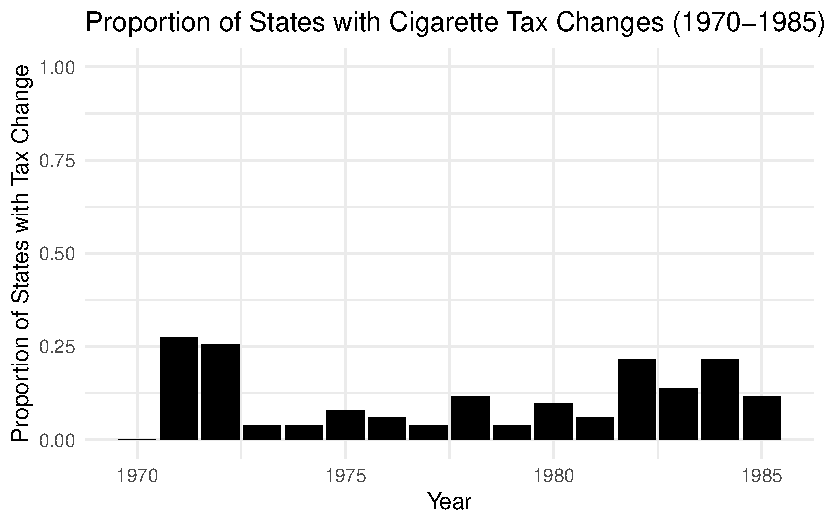
\includegraphics[keepaspectratio]{hwk3-2_files/figure-pdf/Proportion of States with a change in their cigarette tax in each-1.pdf}}

\newpage

\begin{enumerate}
\def\labelenumi{\arabic{enumi}.}
\setcounter{enumi}{1}
\tightlist
\item
  Plot on a single graph the average tax (in 2012 dollars) on cigarettes
  and the average price of a pack of cigarettes from 1970 to 2018.
\end{enumerate}

\pandocbounded{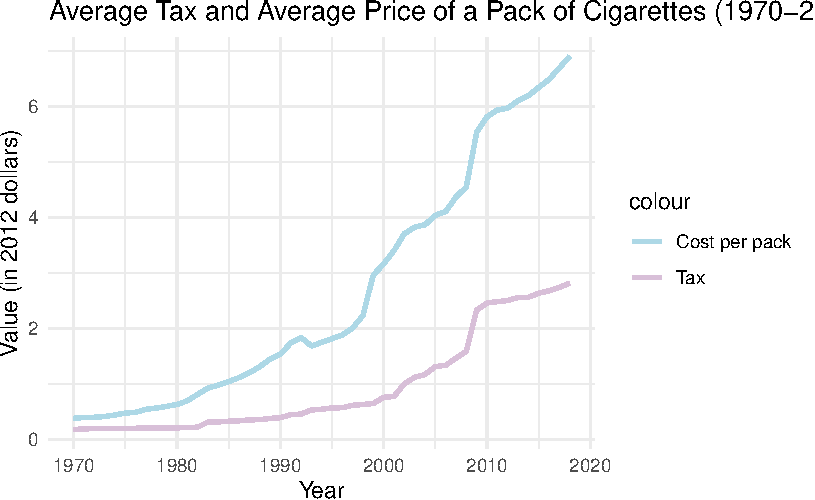
\includegraphics[keepaspectratio]{hwk3-2_files/figure-pdf/unnamed-chunk-3-1.pdf}}

\newpage

\begin{enumerate}
\def\labelenumi{\arabic{enumi}.}
\setcounter{enumi}{2}
\tightlist
\item
  Identify the 5 states with the highest increases in cigarette prices
  (in dollars) over the time period. Plot the average number of packs
  sold per capita for those states from 1970 to 2018.
\end{enumerate}

The states with the highest increases in cigarette prices are:

States with the highest increases in cigarette prices: New York,
District of Columbia, Connecticut, Rhode Island, Massachusetts

\begin{verbatim}
[1] "States with the highest increases in cigarette prices: New York, District of Columbia, Connecticut, Rhode Island, Massachusetts"
\end{verbatim}

\begin{verbatim}
Warning: Using `size` aesthetic for lines was deprecated in ggplot2 3.4.0.
i Please use `linewidth` instead.
\end{verbatim}

\pandocbounded{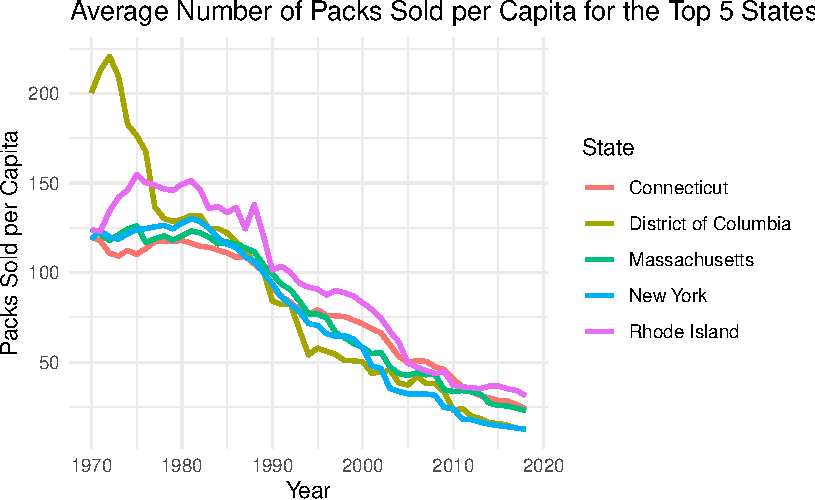
\includegraphics[keepaspectratio]{hwk3-2_files/figure-pdf/unnamed-chunk-4-1.pdf}}

\newpage
4

. Identify the 5 states with the lowest increases in cigarette prices
over the time period. Plot the average number of packs sold per capita
for those states from 1970 to 2018.

The states with the lowest increases in cigarette prices are:

\texttt{r(low\_states\$state,\ collapse\ =\ ",\ "))}

\begin{verbatim}
[1] "States with the lowest increases in cigarette prices: Missouri, North Dakota, Tennessee, Georgia, North Carolina"
\end{verbatim}

\pandocbounded{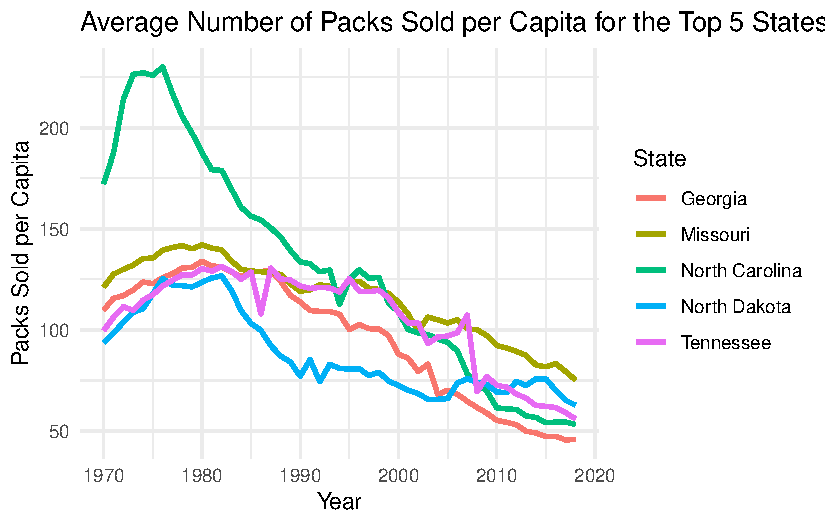
\includegraphics[keepaspectratio]{hwk3-2_files/figure-pdf/unnamed-chunk-5-1.pdf}}

\begin{enumerate}
\def\labelenumi{\arabic{enumi}.}
\setcounter{enumi}{4}
\tightlist
\item
  Compare the trends in sales from the 5 states with the highest price
  increases to those with the lowest price increases.
\end{enumerate}

\begin{verbatim}
`summarise()` has grouped output by 'Year'. You can override using the
`.groups` argument.
\end{verbatim}

\pandocbounded{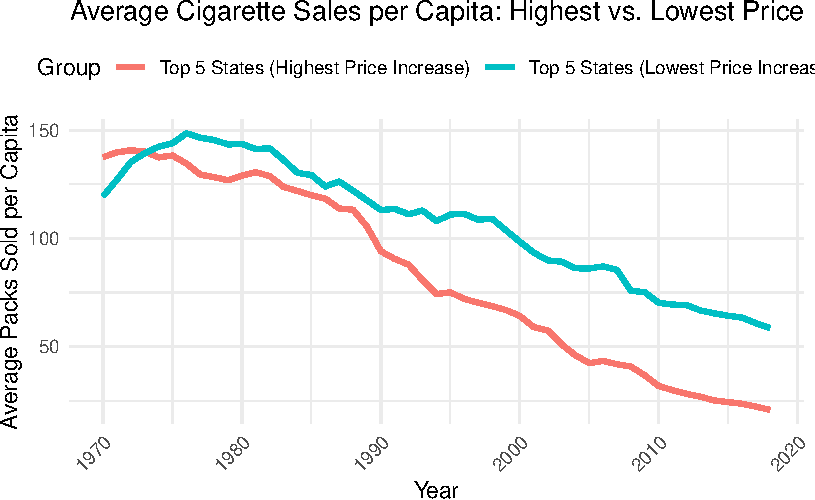
\includegraphics[keepaspectratio]{hwk3-2_files/figure-pdf/unnamed-chunk-6-1.pdf}}

\begin{enumerate}
\def\labelenumi{\arabic{enumi}.}
\setcounter{enumi}{5}
\tightlist
\item
  Focusing only on the time period from 1970 to 1990, regress log sales
  on log prices to estimate the price elasticity of demand over that
  period. Interpret your results.
\end{enumerate}

\begin{Shaded}
\begin{Highlighting}[]
\FunctionTok{modelsummary}\NormalTok{(ols}\FloatTok{.1}\NormalTok{, }\AttributeTok{output =} \StringTok{"markdown"}\NormalTok{)}
\end{Highlighting}
\end{Shaded}

\begin{table}
\centering
\begin{tblr}[         %% tabularray outer open
]                     %% tabularray outer close
{                     %% tabularray inner open
colspec={Q[]Q[]},
column{2}={}{halign=c,},
column{1}={}{halign=l,},
hline{6}={1,2}{solid, black, 0.05em},
}                     %% tabularray inner close
\toprule
& (1) \\ \midrule %% TinyTableHeader
(Intercept) & 5.429 \\
& (0.030) \\
ln_price_cpi & -0.809 \\
& (0.038) \\
Num.Obs. & 1071 \\
R2 & 0.294 \\
R2 Adj. & 0.293 \\
AIC & -522.8 \\
BIC & -512.8 \\
RMSE & 0.19 \\
Std.Errors & IID \\
\bottomrule
\end{tblr}
\end{table}

\begin{enumerate}
\def\labelenumi{\arabic{enumi}.}
\setcounter{enumi}{6}
\tightlist
\item
  Again limiting to 1970 to 1990, regress log sales on log prices using
  the total (federal and state) cigarette tax (in dollars) as an
  instrument for log prices. Interpret your results and compare your
  estimates to those without an instrument. Are they different? If so,
  why?
\end{enumerate}

\begin{Shaded}
\begin{Highlighting}[]
\FunctionTok{modelsummary}\NormalTok{(ivs}\FloatTok{.1}\NormalTok{, }\AttributeTok{output =} \StringTok{"markdown"}\NormalTok{)}
\end{Highlighting}
\end{Shaded}

\begin{table}
\centering
\begin{tblr}[         %% tabularray outer open
]                     %% tabularray outer close
{                     %% tabularray inner open
colspec={Q[]Q[]},
column{2}={}{halign=c,},
column{1}={}{halign=l,},
hline{6}={1,2}{solid, black, 0.05em},
}                     %% tabularray inner close
\toprule
& (1) \\ \midrule %% TinyTableHeader
(Intercept) & 5.418 \\
& (0.055) \\
fit_ln_price_cpi & -0.796 \\
& (0.071) \\
Num.Obs. & 1071 \\
R2 & 0.294 \\
R2 Adj. & 0.293 \\
AIC & -522.7 \\
BIC & -512.7 \\
RMSE & 0.19 \\
Std.Errors & IID \\
\bottomrule
\end{tblr}
\end{table}

\begin{enumerate}
\def\labelenumi{\arabic{enumi}.}
\setcounter{enumi}{7}
\tightlist
\item
  Show the first stage and reduced-form results from the instrument.
\end{enumerate}

First Stage:

\begin{Shaded}
\begin{Highlighting}[]
\FunctionTok{modelsummary}\NormalTok{(first\_stage}\FloatTok{.1}\NormalTok{, }\AttributeTok{output =} \StringTok{"markdown"}\NormalTok{)}
\end{Highlighting}
\end{Shaded}

\begin{table}
\centering
\begin{tblr}[         %% tabularray outer open
]                     %% tabularray outer close
{                     %% tabularray inner open
colspec={Q[]Q[]},
column{2}={}{halign=c,},
column{1}={}{halign=l,},
hline{6}={1,2}{solid, black, 0.05em},
}                     %% tabularray inner close
\toprule
& (1) \\ \midrule %% TinyTableHeader
(Intercept) & 0.841 \\
& (0.005) \\
ln_total_tax & 0.260 \\
& (0.012) \\
Num.Obs. & 1071 \\
R2 & 0.290 \\
R2 Adj. & 0.289 \\
AIC & -1375.2 \\
BIC & -1365.3 \\
RMSE & 0.13 \\
Std.Errors & IID \\
\bottomrule
\end{tblr}
\end{table}

Reduced Form:

\begin{Shaded}
\begin{Highlighting}[]
\FunctionTok{modelsummary}\NormalTok{(reduced}\FloatTok{.1}\NormalTok{, }\AttributeTok{output =} \StringTok{"markdown"}\NormalTok{)}
\end{Highlighting}
\end{Shaded}

\begin{table}
\centering
\begin{tblr}[         %% tabularray outer open
]                     %% tabularray outer close
{                     %% tabularray inner open
colspec={Q[]Q[]},
column{2}={}{halign=c,},
column{1}={}{halign=l,},
hline{6}={1,2}{solid, black, 0.05em},
}                     %% tabularray inner close
\toprule
& (1) \\ \midrule %% TinyTableHeader
(Intercept) & 4.749 \\
& (0.009) \\
ln_total_tax & -0.207 \\
& (0.021) \\
Num.Obs. & 1071 \\
R2 & 0.082 \\
R2 Adj. & 0.082 \\
AIC & -242.0 \\
BIC & -232.1 \\
RMSE & 0.22 \\
Std.Errors & IID \\
\bottomrule
\end{tblr}
\end{table}

\begin{enumerate}
\def\labelenumi{\arabic{enumi}.}
\setcounter{enumi}{8}
\tightlist
\item
  Repeat questions 1-3 focusing on the period from 1991 to 2015.
\end{enumerate}

OLS Regression:

\begin{Shaded}
\begin{Highlighting}[]
\FunctionTok{modelsummary}\NormalTok{(ols}\FloatTok{.2}\NormalTok{, }\AttributeTok{output =} \StringTok{"markdown"}\NormalTok{)}
\end{Highlighting}
\end{Shaded}

\begin{table}
\centering
\begin{tblr}[         %% tabularray outer open
]                     %% tabularray outer close
{                     %% tabularray inner open
colspec={Q[]Q[]},
column{2}={}{halign=c,},
column{1}={}{halign=l,},
hline{6}={1,2}{solid, black, 0.05em},
}                     %% tabularray inner close
\toprule
& (1) \\ \midrule %% TinyTableHeader
(Intercept) & 5.662 \\
& (0.036) \\
ln_price_cpi & -0.997 \\
& (0.025) \\
Num.Obs. & 1275 \\
R2 & 0.561 \\
R2 Adj. & 0.561 \\
AIC & 516.0 \\
BIC & 526.3 \\
RMSE & 0.30 \\
Std.Errors & IID \\
\bottomrule
\end{tblr}
\end{table}

IV Regression:

\begin{Shaded}
\begin{Highlighting}[]
\FunctionTok{modelsummary}\NormalTok{(ivs}\FloatTok{.2}\NormalTok{, }\AttributeTok{output =} \StringTok{"markdown"}\NormalTok{)}
\end{Highlighting}
\end{Shaded}

\begin{table}
\centering
\begin{tblr}[         %% tabularray outer open
]                     %% tabularray outer close
{                     %% tabularray inner open
colspec={Q[]Q[]},
column{2}={}{halign=c,},
column{1}={}{halign=l,},
hline{6}={1,2}{solid, black, 0.05em},
}                     %% tabularray inner close
\toprule
& (1) \\ \midrule %% TinyTableHeader
(Intercept) & 5.882 \\
& (0.041) \\
fit_ln_price_cpi & -1.150 \\
& (0.028) \\
Num.Obs. & 1275 \\
R2 & 0.548 \\
R2 Adj. & 0.548 \\
AIC & 554.0 \\
BIC & 564.3 \\
RMSE & 0.30 \\
Std.Errors & IID \\
\bottomrule
\end{tblr}
\end{table}

First Stage:

\begin{Shaded}
\begin{Highlighting}[]
\FunctionTok{modelsummary}\NormalTok{(first\_stage}\FloatTok{.2}\NormalTok{, }\AttributeTok{output =} \StringTok{"markdown"}\NormalTok{)}
\end{Highlighting}
\end{Shaded}

\begin{table}
\centering
\begin{tblr}[         %% tabularray outer open
]                     %% tabularray outer close
{                     %% tabularray inner open
colspec={Q[]Q[]},
column{2}={}{halign=c,},
column{1}={}{halign=l,},
hline{6}={1,2}{solid, black, 0.05em},
}                     %% tabularray inner close
\toprule
& (1) \\ \midrule %% TinyTableHeader
(Intercept) & 1.316 \\
& (0.004) \\
ln_total_tax & 0.514 \\
& (0.007) \\
Num.Obs. & 1275 \\
R2 & 0.812 \\
R2 Adj. & 0.812 \\
AIC & -1292.8 \\
BIC & -1282.5 \\
RMSE & 0.15 \\
Std.Errors & IID \\
\bottomrule
\end{tblr}
\end{table}

Reduced Form:

\begin{Shaded}
\begin{Highlighting}[]
\FunctionTok{modelsummary}\NormalTok{(reduced}\FloatTok{.2}\NormalTok{, }\AttributeTok{output =} \StringTok{"markdown"}\NormalTok{)}
\end{Highlighting}
\end{Shaded}

\begin{table}
\centering
\begin{tblr}[         %% tabularray outer open
]                     %% tabularray outer close
{                     %% tabularray inner open
colspec={Q[]Q[]},
column{2}={}{halign=c,},
column{1}={}{halign=l,},
hline{6}={1,2}{solid, black, 0.05em},
}                     %% tabularray inner close
\toprule
& (1) \\ \midrule %% TinyTableHeader
(Intercept) & 4.368 \\
& (0.008) \\
ln_total_tax & -0.591 \\
& (0.013) \\
Num.Obs. & 1275 \\
R2 & 0.607 \\
R2 Adj. & 0.607 \\
AIC & 376.2 \\
BIC & 386.5 \\
RMSE & 0.28 \\
Std.Errors & IID \\
\bottomrule
\end{tblr}
\end{table}

Estimates from Questions 6-9

\begin{table}[!h]
\centering\centering
\begin{tabular}[t]{lcccc}
\toprule
\multicolumn{1}{c}{ } & \multicolumn{2}{c}{1970-1990} & \multicolumn{2}{c}{1991-2015} \\
\cmidrule(l{3pt}r{3pt}){2-3} \cmidrule(l{3pt}r{3pt}){4-5}
  & OLS & IV & OLS  & IV \\
\midrule
\addlinespace[0.5em]
\multicolumn{5}{l}{\textit{Estimates}}\\
\midrule \hspace{1em}Log Price & -0.809 & -0.796 & -0.997 & -1.150\\
\hspace{1em} & (0.038) & (0.071) & (0.025) & (0.028)\\
\hspace{1em}N & 1,071 & 1,071 & 1,275 & 1,275\\
\addlinespace[0.5em]
\multicolumn{5}{l}{\textit{Reduced Form}}\\
\midrule \hspace{1em}Log Tax &  & -0.207 &  & -0.591\\
\hspace{1em} &  & (0.021) &  & (0.013)\\
\hspace{1em}N &  & 1,071 &  & \vphantom{1} 1,275\\
\addlinespace[0.5em]
\multicolumn{5}{l}{\textit{First Stage}}\\
\midrule \hspace{1em}Log Tax &  & 0.260 &  & 0.514\\
\hspace{1em} &  & (0.012) &  & (0.007)\\
\hspace{1em}N &  & 1,071 &  & 1,275\\
\bottomrule
\end{tabular}
\end{table}

\begin{enumerate}
\def\labelenumi{\arabic{enumi}.}
\setcounter{enumi}{9}
\tightlist
\item
  Compare your elasticity estimates from 1970-1990 versus those from
  1991-2015. Are they different? If so, why?
\end{enumerate}

1970-1990 shows a positive elasticity (i.e., price increase leads to
more sales), which is unusual for most markets but could be explained by
certain market factors like tax increases, changes in policy (e.g.,
tobacco taxation), or other structural shifts. For instance, if a tax
increase made the product appear more ``exclusive'' or ``prestigious,''
people might have bought more despite the higher price.

1991-2015 shows the more typical negative elasticity, where higher
prices are associated with lower sales. This is consistent with standard
economic theory and consumer behavior, where higher prices lead to a
reduction in demand.




\end{document}
